\section{Integration of Trace\textit{a} in the Capra solution}\label{sec:extension}
\sideboxbegin{o}
This section depicts how the protocol from Section \ref{sec:protocol-extension} has been applied to extend Capra. It describes how to foster trace quality, details the new features and their benefits, the nature of changes made, as well as the potential impact such changes may propagate.
\sideboxend

As we have seen, Capra does not offer any means to address the variation in quality of trace artefacts. This is a recurring limitation for which we propose a meta-description and sketched a protocol to integrate it. 

In this section the module from Trace\textit{a} that tackles quality issue is integrated into Capra following the protocol presented in Section \ref{sec:protocol-extension}.
We first introduce the integration of trace quality into Capra's traceability information metamodel (the localisation of conceptual changes). Then we show the modifications we carried out: the injection of quality features into the core package of Capra and its propagation to the other modules. 
Finally, we uncover the new features allowed by these changes (UI augmentation).
The implementation of such changes impacts the quality of the overall Capra solution. We depict these concerns as well as potential future work at the end of the section.


\subsection{Add trace quality to Capra's metamodel}
We address the lack of quality assessment of trace elements by hacking the customization mechanism of Capra. We integrate Trace\textit{a}, our metamodel for traceability \cite{batot2021-not-another-metamodel}, into Capra as a custom metamodel\footnote{As explained in \url{https://wiki.eclipse.org/Capra/CustomTraceabilityMetaModel}}. To do so, we adapt Trace\textit{a} to fit with Capra's requirements and translate it as an XCore project. 

\subsubsection{Trace model, relationships, and agency}
As can be seen in Listing \ref{lst:traces}, at the root of the Ecore model, a trace model is defined with links and agents. All concepts (except for the model) derive from \texttt{TracingElement}. They have a unique ID and a time stamp. They may also refer to which agent is responsible for their creation. An \texttt{Agent} may be a human being (\texttt{HumanAgent}) or a piece of machinery (\texttt{MachineAgent}).
The top level type of the relationships is \texttt{RelatedTo} -- a generic trace link that connects one origin artefact to potentially many targets. 
% either a \texttt{DomainLink} or a \texttt{EngineeringLink} depending if the link represent a relationship in the realm of the model or the one of the modeler, respectively. 
These implementation decisions follow the genericity requirement Capra asks for. Following the declaration of \textit{RelatedTo} any other kind of relationship can be easily derived.
\pagebreak

\begin{center}
\begin{lstlisting}[caption={Confidence and evidences for trustable traceability},label=lst:relationship,style=mystylextext,frame=shadowbox, rulesepcolor=\color{blue}]
Relationship  returns SysML::Relationship :
    'relationship' Identification?
    RelationshipRelatedElements
    RelationshipBody;

OwnedRelationship returns SysML::Relationship :
    'relationship' Identification?
    'to' RelationshipTargetList
    RelationshipBody;

fragment RelationshipRelatedElements 
            returns SysML::Relationship :
    'from' RelationshipSourceList ( 'to' RelationshipTargetList )?
  | 'to' RelationshipTargetList;

fragment RelationshipSourceList returns SysML::Relationship :
    RelationshipSource ( ',' RelationshipSource )*;

fragment RelationshipSource returns SysML::Relationship :
    source += [SysML::Element | QualifiedName];

fragment RelationshipTargetList returns SysML::Relationship :
    RelationshipTarget ( ',' RelationshipTarget )*
;

fragment RelationshipTarget returns SysML::Relationship :
    target += [SysML::Element | QualifiedName];

fragment RelationshipBody returns SysML::Relationship :
    ';' | '{' RelationshipOwnedElement* '}';

fragment RelationshipOwnedElement returns SysML::Relationship:
      ownedRelatedElement += OwnedRelatedElement
    | ownedRelationship += OwnedDocumentation
    | ownedRelationship += OwnedTextualRepresentationAnnotation;

OwnedRelatedElement returns SysML::Element :
      'element' ( humanId = Name )? ElementBody
    | OwnedRelatedRelationship;

OwnedRelatedRelationship returns SysML::Relationship :
    'relationship' ( humanId = Name )? RelationshipBody;
\end{lstlisting}
\end{center}

\subsubsection{Trace confidence and explainability}
Listing \ref{lst:quality}, represents the \texttt{Confidence} value (\ie an estimation of the existence of the link). Trace\textit{a} defines classes for the different kinds of evidences that may testify the value of the confidence. An \texttt{Evidence} can be a textual annotation (\texttt{Annotation-Evidence}), or a \texttt{RuleEvidence} when a link is created automatically, or an \texttt{AIEvidence} when a learning algorithm is used to identify the link. These latter possess attributes to reproduce their execution (\textit{\eg}, the rule, a certain kind of algorithm, the data set used for training).


%\begin{center}
\begin{lstlisting}[caption={Confidence and evidences for trustable traceability},label=lst:quality,style=mystylexcore,frame=shadowbox, rulesepcolor=\color{blue}]
class Confidence extends TracingElement {
	contains Evidence [0..1] evidence
	double value 
}

abstract class Evidence  extends TracingElement {
	String description
	refers TracingElement [0..*] supportingElements 
}

class AIEvidence extends Evidence {
	String algorithm
	String dataSet
	int executionDate
	double precision
	double recall 
}

class RuleEvidence extends Evidence {
	String rule
	int executionDate 
}

class AnnotationEvidence extends Evidence {
	String explanation 
}
\end{lstlisting}
%\end{center}






\subsubsection{Code change requirements}
To integrate the new link types and link attributes to Capra, interfaces must be realized. \Fig{fig:interfaces-realization} shows the relation of these interfaces, the trace model, and the relationships. 
\begin{figure}[h]  
	\centering
	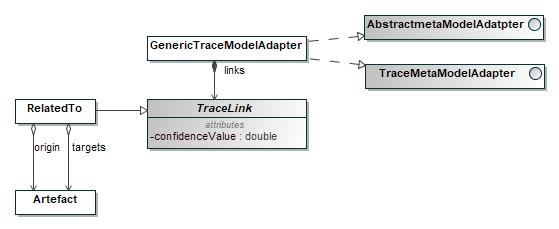
\includegraphics[width=.8\linewidth]{images/interfaces-realization.jpg}
	\caption{Excerpt of the API realization for the definition of trace model and links}
	\label{fig:interfaces-realization} 
\end{figure} 

The interface  \verb|org.eclipse.capra.generic.tracemodel.TraceMetaModelAdapter| must be adapted (see Listing \ref{lst:timapi}) to define generic methods to browse links. The links with their origins and targets are wrapped into \texttt{Connection} to bridge with other packages through ECore reflexion API. Everything is configurable. As long as new link types derive from \texttt{TraceLink}, they will be augmented with quality attributes (\textit{\ie} confidence and evidence).
\begin{lstlisting}[caption={TraceMetaModelAdapter interface},
label=lst:timapi,
style=mystylexcore,
frame=shadowbox, 
rulesepcolor=\color{blue},
morekeywords={class,contains,abstract,extends,\{,\},\[,\],refers,derived,String,get,int,double,List,Connection,EObject,void,String,boolean,Collection,EClass},
linewidth=17.5cm,
xleftmargin=0.3cm
]
EObject createModel();
Collection<EClass> getAvailableTraceTypes(List<EObject> selection);
EObject createTrace(EClass traceType, EObject traceModel, List<EObject> origins, 
    List<EObject> targets);
boolean isThereATraceBetween(EObject origin, EObject target, EObject traceModel);
List<Connection> getConnectedElements(EObject element, EObject traceModel, 
    List<String> traceLinkTypes);
List<Connection> getTransitivelyConnectedElements(EObject element, 
    EObject traceModel, List<String> traceLinkTypes, int transitivityDepth);
List<Connection> getAllTraceLinks(EObject traceModel);
\end{lstlisting}

In the same manner, the interface \verb|org.eclipse.capra.generic.tracemodel.Abstract-| \verb|MetaModelAdapter| offers an interface to define how \textit{internal traces} (\textit{\ie}~links between internal parts of artefacts) must be handled (see Listing \ref{lst:timapi2}).
The default \verb|org.eclipse.generic.trace-| \verb|model.GenericMetaModelAdapter| offers a basic adaptation to these interfaces.

%org.eclipse.capra.core.adapters.TraceMetaModelAdapter



\begin{lstlisting}[caption={AbstractMetaModelAdapter interface},
label=lst:timapi2,
style=mystylexcore,
frame=shadowbox, 
rulesepcolor=\color{blue},
morekeywords={class,contains,abstract,extends,\{,\},\[,\],refers,derived,String,get,int,double,List,Connection,EObject,void,String,boolean,Collection,EClass},
linewidth=17.5cm,
xleftmargin=0.3cm
]
void deleteTrace(List<Connection> toDelete, EObject traceModel);
List<Connection> getInternalElements(EObject element, EObject traceModel, 
    List<String> traceLinkTypes);
List<Connection> getInternalElementsTransitive(EObject element, 
    EObject traceModel, List<String> traceLinkTypes, int transitivityDepth);
boolean isThereAnInternalTraceBetween(EObject first, EObject second);
\end{lstlisting}




 

\subsection{Extend Capra's core interface}
As previously stated, we add a top level link type (\texttt{TraceLink}) to inject the confidence of trace links in Capra. We access the newly added attributes through a reflexive exploration of the trace model structure with \textit{EMF Reflexion} as can be seen in the excerpt in Listing \ref{lst:emfhelper}, from \verb|org.eclipse.capra.core.EMFHelper|.  

%\begin{center}
\begin{lstlisting}[caption={EMFHelper: reflection excerpt for the integration of a confidence value into Capra's \texttt{Connection} interface},
label=lst:emfhelper,
style=mystylexcore,
frame=shadowbox, 
rulesepcolor=\color{blue},
morekeywords={class,contains,abstract,extends,\{,\},\[,\],refers,derived,String,get,int,double,List,Connection,EObject,void,String,boolean,Collection,EClass,EStructuralFeature,return,null,private,static,public,double,for,if},
linewidth=17cm,
xleftmargin=0.3cm
]
public static double getConfidenceValue(EObject tlink) {
    EObject confidenceEO = (EObject)tlink.eGet(
            getEStructuralFeatureByName(tlink, "confidence"));
    if(confidenceEO == null)
        return DEFAULT_CONFIDENCE;
    return (double)confidenceEO.eGet(
            getEStructuralFeatureByName(confidenceEO, "value"));
}

public static EStructuralFeature getEStructuralFeatureByName
                                        (EObject eo, String esfName) {
    for (EStructuralFeature	esf : eo.eClass().getEAllStructuralFeatures()) 
        if(esf.getName().equals(esfName)) 
            return esf;
    return null;
}
\end{lstlisting}
%\end{center}







\subsection{Augment Capra's user experience}
Capra is conceived with the goal to add awareness to its users. Its prime feature is the visualization with textual, graphical, and matrix representations. 
We added features to show and use the confidence in Capra and used it to parameter its user interface, both in textual, graphical, and matrix views. 

\subsubsection{Interactive textual edition}
Based on Eclipse XMI Ecore Model Reflexive Editor, changes in the trace model were integrated automatically. There must be more effort put on insuring the model remains consistent with the different view. \Fig{fig:textext} shows the editor view used for link edition. There, we can see the structure of a link, its confidence value, the evidence associated and potential agents responsible for these elements.\textbf{Edition makes the overall application unstable.}
\begin{figure}[h]  
	\centering
	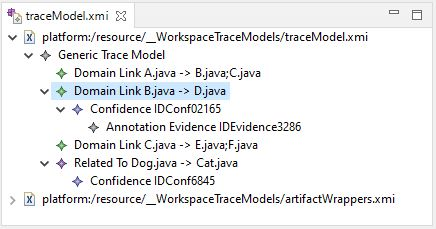
\includegraphics[width=.55\linewidth]{images/textext.JPG}
	\caption{Link structure representation and edition in Eclipse Ecore Model Reflective Editor}
	\label{fig:textext}
\end{figure}





\subsubsection{Matrix UI}
We modified the UI of the association matrix. We use the confidence value to decide weather a cell is green or red. The threshold between the two can be changed through Eclipse interface. \Fig{fig:matrixext} shows an example of the new UI. Red cells reveals "uncertain" links.

\begin{figure}[h]  
	\centering
	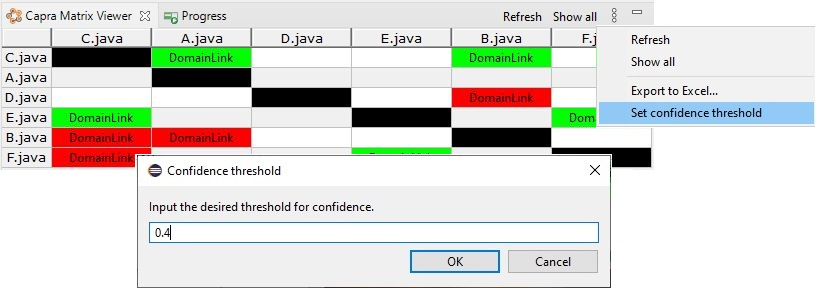
\includegraphics[width=.90\linewidth]{images/matrixViewerExt.JPG}
	\caption{Representation of uncertainty in matrix view}
	\label{fig:matrixext}
\end{figure}

\subsubsection{Plant UML}
We modified the UI of the arrows in PlantUML to show the confidence of a link (when it is not 1.0). {A threshold value for confidence can be set to decide weather a link is shown when transitivity view is \textit{on}.}

\subsection{Change impact evaluation}
The \textit{ad hoc} reflexive exploration that interfaces between the trace metamodel and the core package is the main bottleneck for later maintenance. Its consistency with the structure of a link and the \textit{EObject} wrappers (\texttt{Connection}) that Capra manipulates must be tested when the trace metamodel is modified. 
The choice of this solution is due to the customization mechanism. To allow the redefinition of new types, we can only use the \textit{ExtensionPoint} defined (see Adding a custom Traceability Metamodel\footnote{\url{https://wiki.eclipse.org/Capra/CustomTraceabilityMetaModel}}).

Changes made for the propagation of confidence and its graphical representations of confidence have been posted in a push request to integrate Trace\textit{a} into Capra's branding and thus benefit from its maintenance. The push has been reduced to the minimal introduction of the confidence value for relationships due to the project requirement on genericity.

\subsection{Future work}
We showed the adaptability of Trace\textit{a} and the value of its concepts. Its integration into Capra opens the door to new potential features. 

\begin{descriptioncompact}
    \item[Heat map for matrix view] The matrix representation for tracing are now always considering a Manichean existence / non-existence perception of links. We plan to exploit the confidence value to augment the perception of traceability through a heat map relating confidence levels.
    \item[Uncertainty representation in graphical view] The PlantUML viewer ca be used to plot confidence in other ways than textual or matrix-al. We already integrated a threshold to show only "certain" links, and this research direction could lead to more specific tracing detail .
    \item[PlantUML and Matrix viewer edition of traces] The direct edition of traces and links in the different representations would be a important improvement in the usability of Capra.
    
\end{descriptioncompact}

To operationalize Capra into an industrial environment would require an upgrade of Capra's main design architecture. We develop on Capra's limitation in the next section. 

